% Send to Mandar,Jayesh,Arnab,Deepak and perhaps Rahee
\documentclass{article}
\newcommand{\beq}{\begin{equation}}
\newcommand{\eeq}{\end{equation}}
\newcommand{\ber}{\begin{eqnarray}}
\newcommand{\eer}{\end{eqnarray}}
\newcommand{\nn}{\nonumber}
\newcommand{\dd}[2]{\frac{d}{d{#2}}{(#1)} }
\newcommand{\pdd}[2]{\frac{\partial}{\partial{#2}}{(#1)} }
\usepackage{amsmath}
\usepackage{amsfonts}
\usepackage{url}
\usepackage{graphicx}
\usepackage{caption}
\usepackage{subcaption}
\usepackage{multirow}
\begin{document}
\title{Stiffness parameter identification using Convolutional Neural Networks in TensorFlow}
\author{Nachiket Gokhale\footnote{Conversations with Arnab Majumdar and Mandar Kulkarni are acknowledged and much appreciated.}\\gokhalen@gmail.com}
\date{\today}
\maketitle
\section{Introduction}
We consider a dataset consisting of images of stiffness of the type shown in Figure (\ref{fig:sampleimages}). All images are 32 pixels (x direction) by 128 pixels (y direction). Unlike standard RGB images which have three channels, these images have only one channel (stiffness). So, the shape of each image is $(32,128,1)$. The value of the background stiffness is $1$ and the value of the circle stiffness is a real number which ranges from $2.0$ to $5.0$. Each image contains only one circle or is homogeneous (no circles). That radii of the circles is between $1$ to $3$ pixels both inclusive. Because of the small radii considered, the circles may look like crosses when visualized.\\

We consider the following problems
\begin{enumerate}
\item{\textbf{Binary classification}: Given a stiffness image classify it into homogneous ( no stiff circle, label '0') or having an stiff circle (label '1').}
\item{\textbf{Predicting stiffness location:} Given a stiffness image containing a stiff circle find the x and y coordinates of the center of the stiff circle.}
\item{\textbf{Predicting stiffness value:} Given a stiffness image containing a stiff circle find the value of the stiffness of the circle.}
\item{\textbf{Predicting stiffness radius:} Given a stiffness image containing a stiff circle find the radius of the circle.}
\end{enumerate}
\begin{figure}
  \centering
  \begin{subfigure}[b]{0.45\textwidth}
    \centering
    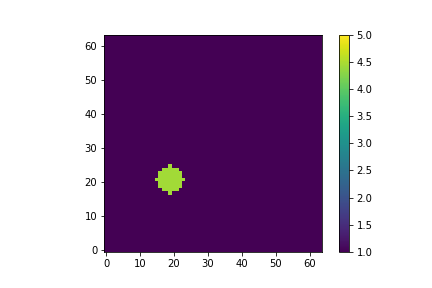
\includegraphics[totalheight=4cm]{circle_id/sample0.png}
    \caption{Sample image 1}
  \end{subfigure}
  %
  \begin{subfigure}[b]{0.45\textwidth}
    \centering
    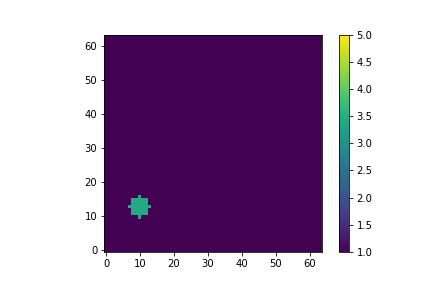
\includegraphics[totalheight=4cm]{circle_id/sample1.png}
    \caption{Sample image 2}
  \end{subfigure}
  %
  \begin{subfigure}[b]{0.45\textwidth}
    \centering
    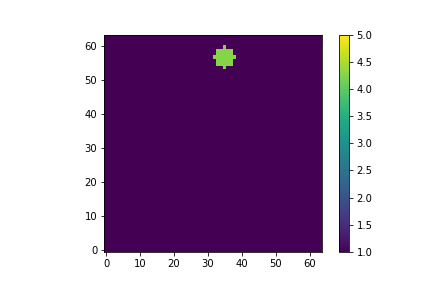
\includegraphics[totalheight=4cm]{circle_id/sample2.png}
    \caption{Sample image 3}
  \end{subfigure}
  \begin{subfigure}[b]{0.45\textwidth}
    \centering
    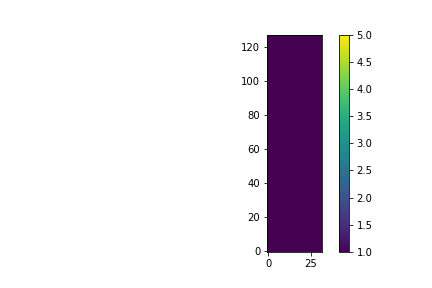
\includegraphics[totalheight=4cm]{circle_id/sample3.png}
    \caption{Sample image 4 (no circle)}
  \end{subfigure}
  %
  \begin{subfigure}[b]{0.45\textwidth}
    \centering
    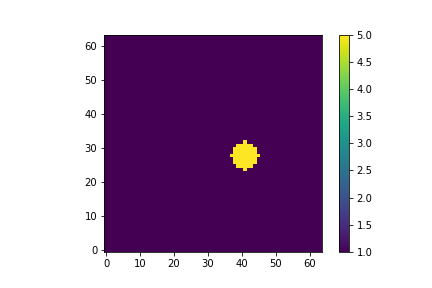
\includegraphics[totalheight=4cm]{circle_id/sample4.png}
    \caption{Sample image 5}
  \end{subfigure}
  %
  \begin{subfigure}[b]{0.45\textwidth}
    \centering
    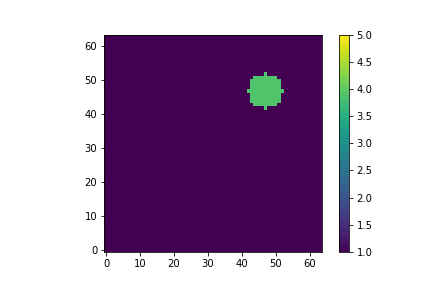
\includegraphics[totalheight=4cm]{circle_id/sample5.png}
    \caption{Sample image 6}
  \end{subfigure}
\caption{\label{fig:sampleimages} Sample images in the image dataset.}
\end{figure}
%
\section{Preliminaries}
We first define the terms '\textbf{epochs}', '\textbf{loss}' or '\textbf{loss function}', '\textbf{min\_delta}' and '\textbf{patience}' and '\textbf{accuracy}'. \\
\begin{enumerate}
\item{'\textbf{epochs}' refers to the number of passes through the training dataset.}
\item{'\textbf{loss}' or '\textbf{loss function}' refers to the cost function being minimized.}
\item{'\textbf{min\_delta}' is the 'minimum change in the monitored quantity to qualify as an improvement, i.e. an absolute change of less than min\_delta, will count as no improvement'. In our case, for 'Binary classification',  the monitored quantity is the validation loss.}
\item{'\textbf{patience}' is the 'number of epochs with no improvement after which training will be stopped'.}
\item{'\textbf{accuracy}' is the ratio of the number of examples classified correctly to the total number of examples.}
\end{enumerate}
\section{Binary classification}
 The parameters used for 'Binary classification' are given in Table (\ref{tab:binaryparam}).We first feature scale the images using their standard deviation and mean using the 'StandardScaler' in 'scikit-learn'. The architecture of the CNN\footnote{This architecture is taken 'as is' from a CNN to classify images into two categories: 'cat' or 'dog'. Ideas for better network architectures are appreciated.} is shown in Figure (\ref{fig:binary_model}). Both the convolutional layers have $32$ filters with a kernel size of $3$. The max-pooling layers have a pool size of $2$ and a stride of $2$. The activation for the output layer is 'sigmoid' and the threshold probability for positive images is $0.5$. The good results that are seen are a consequence of the large number of training parameters. It is also observed that the training of the CNN is quite strongly dependent on the initial random choice of parameters. The metrics for binary classification are shown in Figure (\ref{fig:binarymetrics}). We get an accuracy score of almost $1.0$ right from the start. The confusion matrix is shown in Table (\ref{tab:confusionbinary}). 
\begin{table}
  \centering
  \begin{tabular}{|c|c|}
    \hline
    Parameter & Value \\
    \hline
    Number of training examples   & 1024 \\
    Number of validation examples & 205 \\
    Number of test examples       & 1024 \\
    Maximum number of epochs      & 512 \\
    min{\_}delta      & 10$^{-4}$\\
    patience                      & 10  \\
    Trainable parameters          & 747105\\
    Optimizer         & 'adam'     \\
    Loss function     & 'binary\_crossentropy' \\
    Number of positive training examples (with circle) & 721\\
    Number of negative training examples (without circle) & 303\\
    \hline
  \end{tabular}
  \caption{\label{tab:binaryparam} Parameters for binary classification}
\end{table}
\begin{figure}
   \centering
    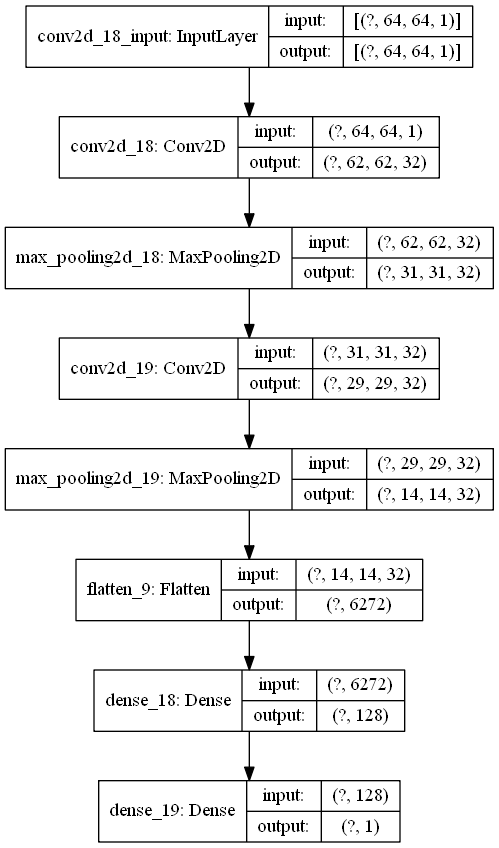
\includegraphics[totalheight=16cm]{circle_id/binary/model.png}
  \caption{\label{fig:binary_model} CNN for binary classification. CNNs for other problems have the same architecture with very minor changes to the output layer.}
\end{figure}
%
\begin{figure}
\centering
\begin{subfigure}[b]{0.45\textwidth}
    \centering
    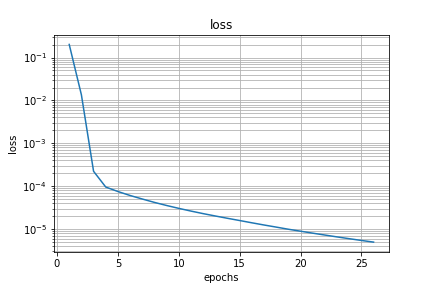
\includegraphics[totalheight=4cm]{circle_id/binary/plotloss.png}
    \caption{Training loss}
  \end{subfigure}
%
\begin{subfigure}[b]{0.45\textwidth}
    \centering
    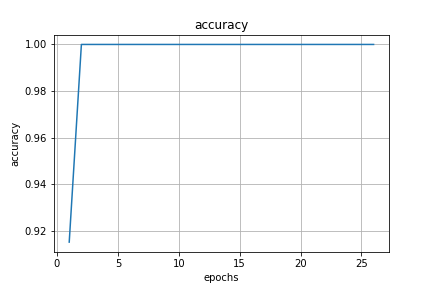
\includegraphics[totalheight=4cm]{circle_id/binary/plotaccuracy.png}
    \caption{Training accuracy}
  \end{subfigure}
%
\begin{subfigure}[b]{0.45\textwidth}
    \centering
    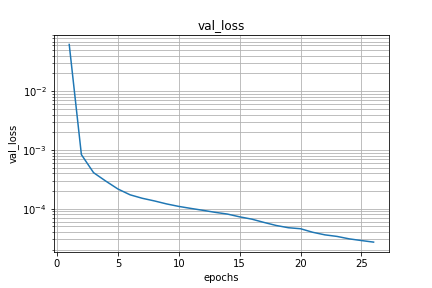
\includegraphics[totalheight=4cm]{circle_id/binary/plotval_loss.png}
    \caption{Validation loss}
  \end{subfigure}
%
\begin{subfigure}[b]{0.45\textwidth}
    \centering
    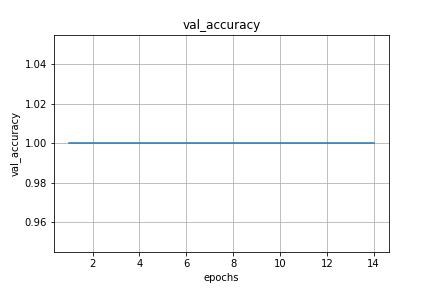
\includegraphics[totalheight=4cm]{circle_id/binary/plotval_accuracy.png}
    \caption{Validation accuracy}
  \end{subfigure}
\caption{\label{fig:binarymetrics} Metrics for binary classification.}
\end{figure}
%
\begin{table}
\begin{center}
  \begin{tabular}{cccc}
    \cline{3-4}
    & & \multicolumn{2}{|c|}{Actual class}  \\
    \cline{3-4}
    & & \multicolumn{1}{|c|}{Circle} &  \multicolumn{1}{|c|}{No Circle}\\
    \hline
    \multicolumn{1}{|c}{Predicted} & \multicolumn{1}{|c|}{Circle} & \multicolumn{1}{|c|}{307} & \multicolumn{1}{|c|}{0} \\
    \cline{2-4}
    \multicolumn{1}{|c}{class} & \multicolumn{1}{|c|}{No circle} & \multicolumn{1}{|c|}{1} & \multicolumn{1}{|c|}{716}\\
    \hline
  \end{tabular}
\end{center}
\caption{\label{tab:confusionbinary} Confusion matrix for binary classification.}
\end{table}
%
\section{Predicting stiffness location}
%
The parameters used for 'Stiffness location' are given in Table (\ref{tab:stifflocparam}). All the images in this dataset are 'positive' i.e. they have a circle present. We first feature scale the images using their standard deviation and mean using the 'StandardScaler' in 'scikit-learn'. We also feature scale the predicted values, because of the range of scales involved. The CNN architecture is the same as the one used in 'Binary classification' shown in Figure (\ref{fig:binary_model}) with the following differences:
\begin{enumerate}
\item{We have two output units instead of one.}
\item{There is no activation for the output layer.}
\end{enumerate}
The training loss and validation loss are shown in Figure (\ref{fig:locationmetrics}) and the errors in location are shown in Figure (\ref{fig:locationerror}). It is seen that for most test examples the error in location is quite small. The absolute error in the x-coordinate is always bounded below 5 pixels and the absolute error in the y-coordinate in 1014 out of 1024 examples is less than 5 pixels. The error in a tiny minority of examples in large (especially in the y coordinate). It would be interesting to see if the model can flag these examples. Perhaps output a measure of 'confidence' in the results.
\begin{table}
  \centering
  \begin{tabular}{|c|c|}
    \hline
    Parameter & Value \\
    \hline
    Number of training examples   & 1024 \\
    Number of validation examples & 205 \\
    Number of training examples   & 1024 \\
    Maximum number of epochs      & 512 \\
    min{\_}delta      & not used\\
    patience                      & not used  \\
    Trainable parameters          & 747,234\\
    Optimizer         & 'adam'     \\
    Loss function     & 'mse' (mean squared error) \\
    \hline
  \end{tabular}
  \caption{\label{tab:stifflocparam} Parameters for stiffness location. Note: early termination was not used. The optimizer was run for the entire $512$ steps.}
\end{table}
%
\begin{figure}
\centering
\begin{subfigure}[b]{0.45\textwidth}
    \centering
    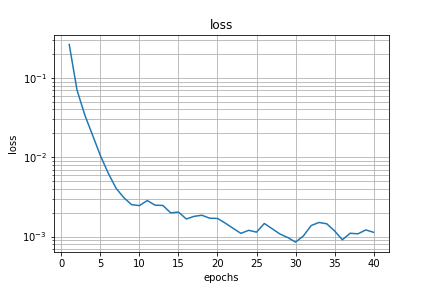
\includegraphics[totalheight=4cm]{circle_id/location/plotloss.png}
    \caption{Training loss}
  \end{subfigure}
%
\begin{subfigure}[b]{0.45\textwidth}
    \centering
    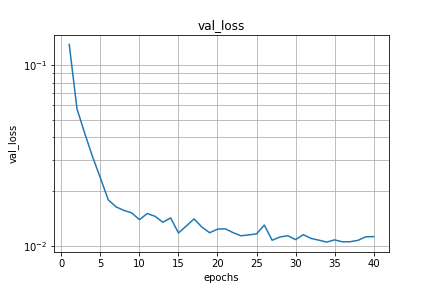
\includegraphics[totalheight=4cm]{circle_id/location/plotval_loss.png}
    \caption{Validation loss}
  \end{subfigure}
%
\caption{\label{fig:locationmetrics} Metrics for stiffness location identification.}
\end{figure}
%
\begin{figure}
\centering
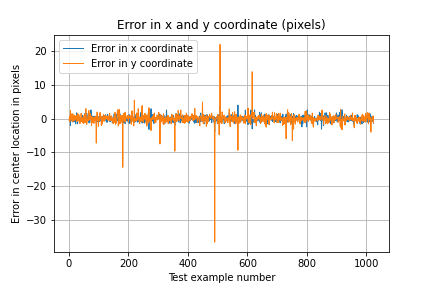
\includegraphics{circle_id/location/plotabserror.png}
\caption{\label{fig:locationerror} Error in pixels for stiffness location identification.}
\end{figure}
%
\section{Predicting stiffness value}
The parameters used for 'Predicting stiffness value' are given in Table (\ref{tab:stiffvalparam}). All the images in this dataset are 'positive' i.e. they have a circle present. We first feature scale the images using their standard deviation and mean using the 'StandardScaler' in 'scikit-learn'. We also feature scale the predicted values, because of the range of scales involved. The CNN architecture is the same as the one used in 'Binary classification' shown in Figure (\ref{fig:binary_model}) with the following difference:
%
\begin{enumerate}
\item{There is no activation for the output layer.}
\end{enumerate}
The training and validation loss are shown in Figure (\ref{fig:stiffvalmetrics}). The absolute and relative error in the stiffness value prediction are shown in Figure (\ref{fig:stiffvalerror}). Most of the test cases (982 out of 1024) show a relative error of less than 10\%. 
%
\begin{table}
  \centering
  \begin{tabular}{|c|c|}
    \hline
    Parameter & Value \\
    \hline
    Number of training examples   & 1024 \\
    Number of validation examples & 205 \\
    Number of training examples   & 1024 \\
    Maximum number of epochs      & 512 \\
    min{\_}delta      & not used\\
    patience                      & not used  \\
    Trainable parameters          & 747,105\\
    Optimizer         & 'adam'     \\
    Loss function     & 'mse' (mean squared error) \\
    \hline
  \end{tabular}
  \caption{\label{tab:stiffvalparam} Parameters for stiffness value identification. Note: early termination was not used. The optimizer was run for the entire $512$ steps.}
\end{table}
%
\begin{figure}
\centering
\begin{subfigure}[b]{0.45\textwidth}
    \centering
    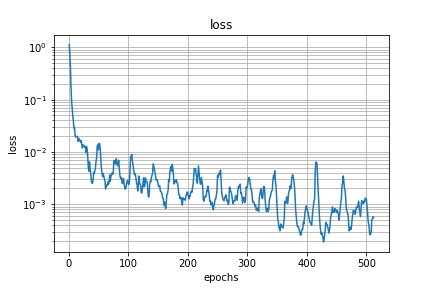
\includegraphics[totalheight=4cm]{circle_id/stiffval/plotloss.png}
    \caption{Training loss}
  \end{subfigure}
%
\begin{subfigure}[b]{0.45\textwidth}
    \centering
    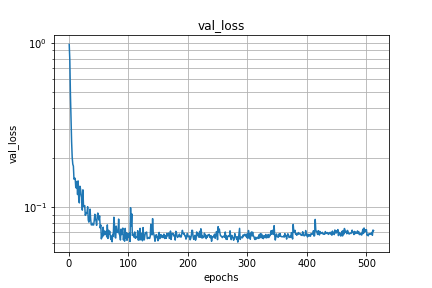
\includegraphics[totalheight=4cm]{circle_id/stiffval/plotval_loss.png}
    \caption{Validation loss}
  \end{subfigure}
%
\caption{\label{fig:stiffvalmetrics} Metrics for stiffness value identification.}
\end{figure}
%
\begin{figure}
  \centering
\begin{subfigure}[b]{0.95\textwidth}
    \centering  
    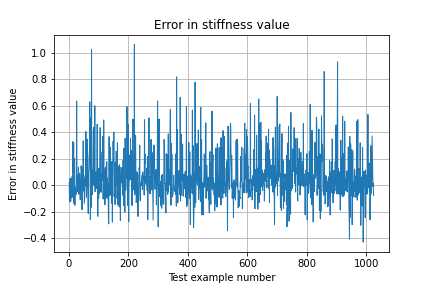
\includegraphics{circle_id/stiffval/plotabserror.png}
    \caption{\label{fig:stiffvalabserror} Error in stiffness value identification.}
\end{subfigure}
\begin{subfigure}[b]{0.95\textwidth}
    \centering  
    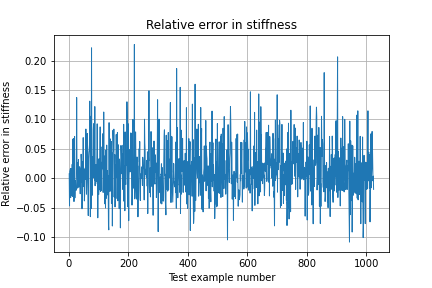
\includegraphics{circle_id/stiffval/plotrelcomparison.png}
    \caption{\label{fig:stiffvalrelerror} Relative error in stiffness value identification.}
\end{subfigure}
\caption{\label{fig:stiffvalerror} Error in stiffness value identification}
\end{figure}
\section{Predicting circle radius}
%
The parameters used for 'Predicting stiffness radius' are given in Table (\ref{tab:stiffradparam}). All the images in this dataset are 'positive' i.e. they have a circle present. We first feature scale the images using their standard deviation and mean using the 'StandardScaler' in 'scikit-learn'. We also feature scale the predicted values, because of the range of scales involved. The CNN architecture is the same as the one used in 'Binary classification' shown in Figure (\ref{fig:binary_model}) with the following difference:
%
\begin{enumerate}
\item{There is no activation for the output layer.}
\end{enumerate}
The training and validation loss are shown in Figure (\ref{fig:stiffradmetrics}). The absolute and relative error in the stiffness radius prediction are shown in Figure (\ref{fig:stiffraderror}). Most of the test cases (868 out of 1024) show a relative error of less than 10\%.
%
\begin{table}
  \centering
  \begin{tabular}{|c|c|}
    \hline
    Parameter & Value \\
    \hline
    Number of training examples   & 1024 \\
    Number of validation examples & 205 \\
    Number of training examples   & 1024 \\
    Maximum number of epochs      & 512 \\
    min{\_}delta      & not used\\
    patience                      & not used  \\
    Trainable parameters          & 747,105\\
    Optimizer         & 'adam'     \\
    Loss function     & 'mse' (mean squared error) \\
    \hline
  \end{tabular}
  \caption{\label{tab:stiffradparam} Parameters for stiffness radius identification. Note: early termination was not used. The optimizer was run for the entire $512$ steps.}
\end{table}
%
\begin{figure}
\centering
\begin{subfigure}[b]{0.45\textwidth}
    \centering
    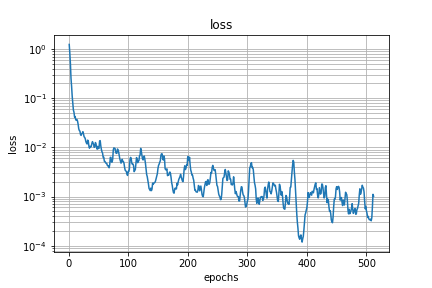
\includegraphics[totalheight=4cm]{circle_id/stiffrad/plotloss.png}
    \caption{Training loss}
  \end{subfigure}
%
\begin{subfigure}[b]{0.45\textwidth}
    \centering
    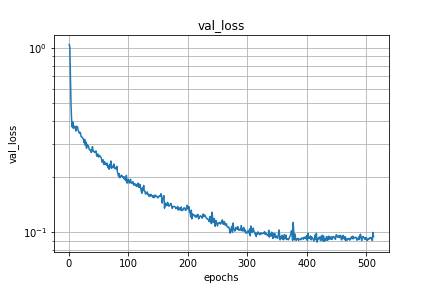
\includegraphics[totalheight=4cm]{circle_id/stiffrad/plotval_loss.png}
    \caption{Validation loss}
  \end{subfigure}
%
\caption{\label{fig:stiffradmetrics} Metrics for stiffness radius identification.}
\end{figure}
%
%
\begin{figure}
  \centering
\begin{subfigure}[b]{0.95\textwidth}
    \centering  
    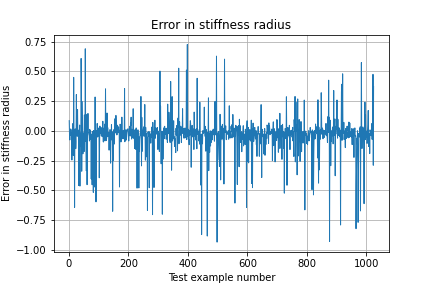
\includegraphics{circle_id/stiffrad/plotabserror.png}
    \caption{\label{fig:stiffradabserror} Error in stiffness radius identification.}
\end{subfigure}
\begin{subfigure}[b]{0.95\textwidth}
    \centering  
    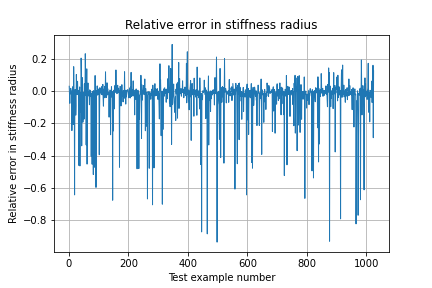
\includegraphics{circle_id/stiffrad/plotrelcomparison.png}
    \caption{\label{fig:stiffradrelerror} Relative error in stiffness radius identification.}
\end{subfigure}
\caption{\label{fig:stiffraderror} Error in stiffness radius identification}
\end{figure}
%
\section{Things to do}
\begin{enumerate}
\item{Checkpoint and save best weights instead of just running for $512$ epochs}
\item{Use prior knowledge to improve performance. e.g. if we know that radius can lie between 1 pixel and 3 pixels we can use that information to improve performence.}
\end{enumerate}
\end{document}
